\usetikzlibrary{shapes,positioning,matrix}
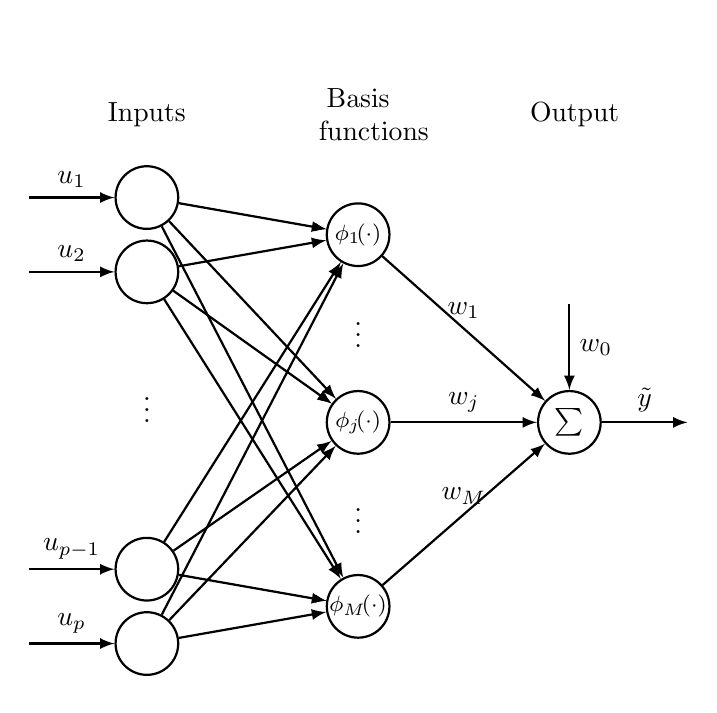
\begin{tikzpicture}[
scale = 1,
plain/.style={
  draw=none,
  fill=none,
  },
net/.style={
  matrix of nodes,
  nodes={
    draw,
    circle,
    thick,
    inner sep=8pt
    },
  nodes in empty cells,
  column sep=0.8cm,
  row sep=-10pt
  },
>=latex
]

\matrix[net] (mat)
{
|[plain]| \parbox{1cm}{\centering Inputs} & 
|[plain]| \parbox{1cm}{\centering Basis\\functions} &
|[plain]| \parbox{1cm}{\centering Output} \\
& |[plain]| \\
|[plain]| & \\
& |[plain]| \\
|[plain]| & |[plain]| $\vdots$ \\
|[plain]| $\vdots$&  &  \\
|[plain]| &  |[plain]|  \\
|[plain]|& |[plain]|$\vdots$ \\
 &  |[plain]|  \\
 |[plain]|&   \\
  &  |[plain]| \\
};

\foreach \ai [count=\mi ]in {2,4}
     \draw[thick][<-] (mat-\ai-1) -- node[above] {$u_\mi$} +(-1.5cm,0);
     \draw[thick][<-] (mat-9-1) -- node[above] {$u_{p-1}$} +(-1.5cm,0);
     \draw[thick][<-] (mat-11-1) -- node[above] {$u_{p}$} +(-1.5cm,0);

\foreach \ai in {2,4,9,11}
{\foreach \aii  in {3,6,10}
  \draw[thick][->] (mat-\ai-1) -- (mat-\aii-2) ;
  
  
}

  \draw[->] (mat-2-1) -- (mat-3-2) node(){\footnotesize $\phi_1\!(\cdot)$};
  \draw [->] (mat-4-1) -- (mat-6-2) node(){\footnotesize$\phi_j\!(\cdot)$};
    \draw [->] (mat-9-1) -- (mat-10-2) node(){\footnotesize$\phi_M\!(\cdot)$};

  \draw[thick][->] (mat-3-2) --node[above]{$w_1$} (mat-6-3)node(){ $\sum$};
  \draw[thick][->] (mat-6-2) --node[above]{$w_j$} (mat-6-3);
  \draw[thick][->] (mat-10-2) --node[above]{$w_M$} (mat-6-3);
  
\draw[thick][->] (mat-6-3) -- node[above] {$\tilde{y}$} +(1.5cm,0);
\draw[thick][<-] (mat-6-3) -- node[right] {$w_0$} +(0,1.5cm);

\end{tikzpicture}